\documentclass[12pt, letterpaper, parskip = full]{article}
\usepackage[mmddyyyy]{datetime}

\usepackage[utf8]{inputenc}
\usepackage{amsmath}
\usepackage{mathpazo}
\usepackage{eulervm}
\usepackage[skip=10pt plus1pt]{parskip}

\usepackage[margin=1in]{geometry}
%\linespread{1.20}
\usepackage{enumerate}
\usepackage{enumitem}
\usepackage{listings}
\usepackage[T1]{fontenc}
\usepackage{amsfonts}
\usepackage{amssymb}
\usepackage{amsthm}
\usepackage{multirow,array}
\usepackage{graphicx}
\usepackage{physics}
\usepackage{bm}
\usepackage{tikz}
\usepackage{breqn}
\usepackage[longnamesfirst]{natbib}
\usepackage{comment}
\usepackage{setspace}
\usepackage{hyperref}
\usepackage{accents}
\usepackage{graphicx}

\graphicspath{{Images/}}
\setlength{\parindent}{0pt}

\newtheorem{theorem}{Theorem}
\newtheorem{corollary}{Corollary}
\newtheorem{lemma}{Lemma}
\newtheorem{definition}{Definition}
\newtheorem{axiom}{Axiom}
\newcommand{\e}{\mathrm{e}}
\newcommand{\Var}{\mathrm{Var}}
\newcommand{\Ex}[1]{\mathbb{E}\left[#1\right]}
\renewcommand{\Pr}[1]{\mathbb{P}(#1)}
\newcommand{\plim}{\mathrm{plim}}
\newcommand{\pc}[1]{\frac{\dot{#1}(t)}{#1(t)}}
\renewcommand\qedsymbol{$\blacksquare$}
\newcommand{\ubar}[1]{\underaccent{\bar}{#1}}

\title{Worksheet 5 \\ Actuarial Corporate Finance}
\author{Alejandro Flores-Brown}

\begin{document}

    \maketitle

    I think the only worksheet problem assigned for homework was the third problem, but I will rewrite the first two just in case.

    \section{Problem 1}

    \subsection{Part 1}

    The risk-free rate is represented by the rate on Treasury bills, which is \(4.8\%\) here; accordingly, the excess return on small stocks is \(\boxed{0.232 - 0.048 = 18.4\%}\)

    \subsection{Part 2}

    The excess return on corporate bonds is \(\boxed{0.075 - 0.048 = 2.7\%}\)

    \subsection{Part 3}

    The market risk premium is approximated by the S\&P 500; accordingly, the excess return is \(\boxed{0.132 - 0.048 = 8.4\%}\)

    \subsection{Part 4}

    Using CAPM, we have
    \[  0.075 = 0.048 + \beta_{CB} (0.132 - 0.048) \implies \boxed{\beta_{CB} = 0.3214}\]

    \subsection{Part 5}

    The relationship between the excess return of the corporate bonds portfolio and the return of the market can be expressed in terms of volatility as
    \[ \Ex{R{CB}} = r_f + \frac{\sigma_{CB}}{\sigma_{M}} (\Ex{R_M} - r_f) \implies \boxed{\sigma_{CB} = \frac{0.084}{0.2 \times 0.027} = 6.43\%}    \]

    \section{Problem 2}

    The current portfolio beta is given by \(\beta_P = 0.6 \times 1.5 + 0.4 \times 1.25 = 1.4\). To lower it to \(0.5\), we need to use a different linear combination of assets. We can get this by writing
    \[ \beta_P = 0.5 = 1.4 w + 0 (1-w) \implies w = \frac{0.5}{1.4} = 0.3571   \]
    As written, \(w\) is the remaining weight on the portfolio, so the percentage invested in the risk-free bond should be \( \boxed{\alpha = 1 - 0.3571 = 0.6429}  \). 

    \section{Problem 3}

    \subsection{Part 1}

    The CAPM gives \( \Ex{R_i} = r_f + \beta{i,M} (\Ex{R_M} - r_f)\). The only difference is \(\beta_{i,M}\), which immediately tells us that the asset with a higher \(\beta\) should have a higher expected return. That means that asset \(A\) has a higher expected return.

    \subsection{Part 2}

    Plugging numbers into the CAPM, we get
    \begin{align*}
        \Ex{R_A} &= 0.03 + 2.1 (0.09 - 0.03) = 15.6\% \\
        \Ex{R_B} &= 0.03 + 0.7 (0.09 - 0.03) = 7.2\%
    \end{align*}

    \subsection{Part 3}
    The portfolio's beta and expected return are given by 
    \begin{align*}
    \Ex{R_{P1}} &= 0.25 \Ex{R_B} + 0.75 \Ex{R_A} = 0.25 \times 0.072 + 0.75 \times 0.156 &= 13.5\% \\
    \beta_{P1} &= 0.25 \times \beta_B + 0.75 \times \beta_A = 0.25 \times 0.7 + 0.75 \times 2.1 &= 1.75
    \end{align*}

    \subsection{Part 4}
    This portfolio's beta and expected return are given by
    \begin{align*}
    \Ex{R_{P2}} &= -0.5 \Ex{R_B} + 1.5 \Ex{R_A} = -0.5 \times 0.072 + 1.5 \times 0.156 &= 19.8\% \\
    \beta_{P2} &= -0.5 \times \beta_B + 1.5 \times \beta_A = -0.5 \times 0.7 + 1.5 \times 2.1 &= 2.8
    \end{align*}
    \subsection{Part 5}

    The assets clearly lie along a straight line. With a quick and dirty Julia script:

    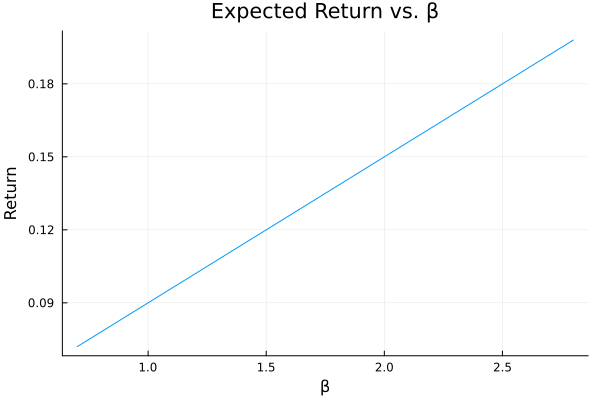
\includegraphics[scale=0.5]{hw5_plot.png}

    \begin{verbatim}
    using Plots

    R = [0.156, 0.072, 0.135, 0.198]
    beta = [2.1, 0.7, 1.75, 2.8]

    betarplot = plot(beta, R, xlabel = "beta", ylabel = "Return", 
    title = "Expected Return vs. beta", legend = false)
    #definitely a straight line
    png(betarplot, "ws5_plot")

    \end{verbatim}

\end{document}